% Machine translated from the Danish original, ../danish/dma-problems-2026-trial.tex
\noindent\emph{This problem set has been machine translated from the Danish original.}
\medskip

\section*{Multiple-choice}\label{sec:mc}

\placeholder{Where to enter the multiple-choice answers, e.g.\ the multiple-choice module of the exam system.}

\multiplechoicestart



\question{Arrays}
Let \(A[0:4] = \langle 8, 2, 9, 5, 4 \rangle\) and \(B[1:5] = \langle 5, 4, 1, 2, 3 \rangle\).
What is \(A[3 \cdot B[4]-3]\)?
\oneanswer

\optionsstart
\answer \(2\)
\answer \(4\)
\answer \(5\) \correct
\answer \(8\)
\answer \(9\)
\optionsend
\explanation{
  We first find \(B[4]\), which is \(2\).
  We then find \(A[3 \cdot B[4] - 3] = A[3] \),
  which is \(5\).
}

\question{Peaks in an array}
Which indices are peaks in the following array: \(A[0:4] = [2,8,8,9,1]\)?
Recall that an index \(i\) is a peak if \(A[i]\) is greater than or equal to all of its neighboring elements (each element has one or two neighbors).
\multipleanswers
\optionsstart
\answer \(0\)
\answer \(1\) \correct
\answer \(2\)
\answer \(3\) \correct
\answer \(4\)
\optionsend
\explanation{
  Here \(A[1]=8\) is greater than \(A[0]=2\) and equal to \(A[2]=8\),
  and \(A[3]=9\) is greater than \(A[2]=8\) and \(A[4]=1\).
  Hence \(1\) and \(3\) are peaks.
}

\question{Combinatorics}
In how many different ways can we choose \(k\) elements from a set with
\(n\) elements, when the order does not matter and we may not choose the same element
more than once?
\oneanswer
\optionsstart
\answer \(n^{k}\)
\answer \(\frac{n!}{(n-k)!}\)
\answer \(\frac{n!}{(n-k)!k!}\) \correct
\answer \(n \cdot \sum_{i=1}^{k} i\)
\optionsend
\explanation{
The correct answer is the binomial coefficient \(\binom{n}{k} = \frac{n!}{(n-k)!k!}\), which is exactly the number of subsets of size $k$ of a set of size $n$.
}


\question{Hashing}
Which of the following properties are desirable for a hash function?
\multipleanswers
\optionsstart
\answer Every key is equally likely to be mapped to each entry of the hash table, independently of where the other keys are mapped. \correct
\answer The hash function is continuous.
\answer If you compute the hash value of the same key several times,
you almost always get different results.
\answer The hash function is fast to compute. \correct
\optionsend
\explanation{
\begin{enumerate}

    \item We want the keys to be spread evenly over the hash table, and the positions of the keys should not depend on each other,
so we want property (1).
\item We gain nothing from continuity of a hash function,
so (2) is irrelevant.
\item A hash function must always give the same result for the same key,
so (3) is wrong.
\item Finally, we want the hash function to be fast to compute,
so (4) is correct.
\end{enumerate}
}


\question{Graph concepts}
Which of the following concepts can be used to describe parts of a graph $G=(V,E)$?
\multipleanswers
\optionsstart
\answer Edges \correct
\answer Cycles \correct
\answer Axes
\answer Paths \correct
\answer Curves
\answer Functions
\optionsend
\explanation{
A graph consists of vertices and edges.
One can also speak of paths and cycles in a graph.
Concepts such as axes, curves and functions do not belong to basic graph theory.
}


\question{Basic pseudocode keywords}
Which of the following words do we often use in pseudocode?
\multipleanswers
\optionsstart
\answer if \correct
\answer can
\answer for \correct
\answer return \correct
\answer invert
\answer align
\optionsend
\explanation{
In standard pseudocode we often use if, for and return, but not the other words.
}

\question{Data structures from the syllabus}
Which of the following are names of data structures from the course syllabus?
\multipleanswers
\optionsstart
\answer extended pointer
\answer queue \correct
\answer collection
\answer double chain
\answer family
\answer singly linked list \correct
\optionsend
\explanation{
Singly linked lists and queues are classic data structures in the syllabus. Terms such as extended pointer, collection, double chain and family are not standard data structures in the course.
}


\question{Properties of binary search trees}
Which of the following statements describe properties of a binary search tree?
\multipleanswers
\optionsstart
\answer Each node has zero, one or two children \correct
\answer Each node has two parents
\answer For every node $v$, if $v.left \neq \text{NIL}$, then $v.left.key \leq v.key$ \correct
\answer The height of the tree (i.e.,~the number of edges on the longest path from a leaf to the root) is always $O(\log n)$, where $n$ is the number of nodes
\answer The number of nodes in the left subtree of the root is always smaller than the number in the right subtree
\optionsend
\explanation{
A binary search tree has at most two children per node, and the key of the left child is less than or equal to the key of the node. The numbers of nodes in the left and right subtrees can vary, so the left subtree does not always have fewer nodes. The height is not always $O(\log n)$; this only holds for balanced trees.
Every node has exactly one parent, except the root, which has none.
}


\question{Properties of relations}
Which of the following words describe a property of a relation?
\multipleanswers
\optionsstart
\answer reflexive \correct
\answer indicative
\answer bi-implicative
\answer transitive \correct
\answer projective
\answer distributive
\optionsend
\explanation{
The words reflexive and transitive describe properties of relations.
Words such as indicative, bi-implicative, projective and distributive are not standard properties of relations.
}


\question{Symmetric relation}
Let $X$ be a set and let $R \subseteq X \times X$ be a relation on $X$.
What is the definition of $R$ being symmetric?
\oneanswer
\optionsstart
\answer If $(a,b) \in R$, then $(a,a) \in R$
\answer If $(a,b) \in R$, then $(a,c) \in R$ for all $c \in X$
\answer If $(a,b) \in R$, then $(b,a) \in R$ and $a \neq b$
\answer If $(a,b) \in R$, then $(b,a) \in R$ \correct
\optionsend
\explanation{
A relation $R$ is symmetric if for all $a,b \in X$: $(a,b) \in R \implies (b,a) \in R$.
The other statements do not describe symmetry.
}

\question{Asymptotic analysis}
Consider the function
\begin{align*}
  f(x) = x^{3}\log x + 7x^{2} + 10x.
\end{align*}
Which of the following statements about \(f\) are correct?
\multipleanswers
\optionsstart
\answer \(f = O(x^{3})\)
\answer \(f = O(x^{3}\log x)\) \correct
\answer \(f = O(x^{4})\) \correct
\answer \(f = \Omega(x^{3})\) \correct
\answer \(f = \Omega(x^{4})\)
\answer \(f = \Theta(x^{3}\log x)\) \correct
\answer \(f = \Theta(x^{3})\)
\optionsend
\explanation{
  The dominant term of \(f\) is \(x^{3}\log x\),
  so \(f = O(x^{3}\log x)\) and \(f = O(x^{4})\).
  Since \(f\) grows faster than \(x^{3}\), we have \(f = \Omega(x^{3})\).
  Since the dominant term is \(x^{3}\log x\), we have \(f = \Theta(x^{3}\log x)\).
}

\question{Pseudocode}
Consider the following pseudocode
\begin{codebox}
\Procname{$\proc{While-Loop}(x)$}
\li $y \gets 2 \cdot x$
\li $S \gets 0$
\li \While $y > 1$ \Do
\li \(S \gets 2 \cdot S + y\)
\li \(y \gets y-2\)
    \End
\li \Return S
\end{codebox}
What is returned when the code is called with input $x=3$?
\oneanswer
\optionsstart
\answer 3
\answer 12
\answer 25
\answer 34 \correct
\answer 42
\optionsend
\explanation{Before the while loop we have $y=6$ and $S=0$. Then the following happens in each iteration:
\begin{itemize}
    \item Iteration 1: $S=0\cdot 2+6=6$, $y=6-2=4$
    \item Iteration 2: $S=6\cdot 2+4=16$, $y=4-2=2$
    \item Iteration 3: $S=16\cdot 2+2=34$, $y=2-2=0$
\end{itemize}
}

\question{RAM model}
Which of the following operations take constant time in the RAM model?
Assume that \(a,b\) are integer variables and \(A\) is an array.
\multipleanswers

\optionsstart
\answer \(b = \sum_{i=1}^{n} A[i]\)
\answer \(b - a\) \correct
\answer \(b = A[3]\) \correct
\answer \(b = A[a^{3}]\) \correct
\answer \(b = A[b^{a}]\)
\optionsend
\explanation{
  \begin{itemize}
      \item  The first operation takes \(O(n)\) time, since both an addition and an array lookup must be performed \(n\) times.
      \item  A subtraction takes constant time \(O(1)\).
      \item A single lookup in $A$ takes $O(1)$ time.
      \item  \(a^{3}\) is a constant number of multiplications, so the lookup $A[a^3]$
        also takes constant time \(O(1)\).
      \item  \(b^{a}\) may take \(\log a\) multiplications in the worst case.
  \end{itemize}
}




\question{Sets and integers}
Let $A = \{5, 10, 2026\}$ and $B = \{5k \mid k \in \{1,\dots,500\}\}$.
Which of the following statements are true?
\multipleanswers
\optionsstart
\answer $\sum_{a \in A} a = 2041$ \correct
\answer $\text{GCD}(B) = 2500$
\answer $\sum_{b \in B-A} b=\sum_{b \in B} b-\sum_{a \in A} a$
\answer $A \subseteq B$
\answer $\sum_{b \in B} b = 5\cdot 250\cdot 501$ \correct
\optionsend
\explanation{
$\sum_{a \in A} a=5+10+2026=2041$.
$\text{GCD}(B)=5$.
$\sum_{b \in B-A} b=\sum_{b \in B} b-5-10$; we should not subtract 2026 as is done in the expression $\sum_{b \in B} b-\sum_{a \in A} a$.
Since $2026\notin B$, it is not the case that $A \subseteq B$.
We have $\sum_{b \in B} b=\sum_{k=1}^{500} 5k=5\sum_{k=1}^{500} k=5\cdot 250\cdot 501$.
}

\question{Modular arithmetic}
Recall that for integers $a$ and $n$ we use the notation $a\text{ mod }n$ to denote the remainder of \(a\) modulo \(n\).
What is the value of the following expression?
\begin{align*}
  (58\text{ mod }8) \cdot \left((5214\text{ mod }4)+ (8627\text{ mod }5)\right)
\end{align*}
\oneanswer
\optionsstart
\answer \(0\)
\answer \(2\)
\answer \(6\)
\answer \(8\) \correct
\answer \(10\)
\optionsend
\explanation{
We have \(58\text{ mod }8 = 2\), \(5214\text{ mod }4 = 2\) and \(8627\text{ mod }5 = 2\).
So the expression evaluates to \(2 \cdot (2 + 2) = 8\).
}

\question{Negation of statements}
What is the negation of the following statement?
\begin{align*}
  \forall x \in X \; \exists y \in Y : y \mid x^{2}.
\end{align*}
\oneanswer

\optionsstart
\answer \(\forall x \in X \; \forall y \in Y : y \nmid x^{2}\)
\answer \(\forall x \in X \; \exists y \in Y : y \nmid x^{2}\)
\answer \(\exists x \in X \; \exists y \in Y : y \nmid x^{2}\)
\answer \(\exists x \in X \; \forall y \in Y : y \nmid x^{2}\) \correct
\optionsend
\explanation{
  To negate the statement, every \(\exists\)
  is changed into \(\forall\) and vice versa, and the inner statement \(y \mid x^{2}\)
  is negated, which gives \(y \nmid x^{2}\).
}

\question{Max-Heap}
You run BUILD-MAX-HEAP on the array \(A = \langle 3, 1, 6, 5, 2, 4 \rangle\).
Which heap do you get as the result?
\oneanswer

\optionsstart
\answer \(\langle 6, 4, 5, 1, 2, 3 \rangle\)
\answer \(\langle 6, 5, 4, 1, 2, 3 \rangle\) \correct
\answer \(\langle 6, 5, 4, 3, 2, 1 \rangle\)
\answer \(\langle 6, 5, 3, 1, 2, 4 \rangle\)
\answer \(\langle 6, 3, 4, 5, 2, 1 \rangle\)
\optionsend
\explanation{
  When BUILD-MAX-HEAP is run bottom-up on the array, the largest value is moved to the root,
  and the heap property is restored recursively for all subtrees.
  The final array is \(\langle 6, 5, 4, 1, 2, 3 \rangle\), where no node
  has a child with a larger value than itself.
}



\question{Array representation of a linked list}
Which singly linked list \(L\) is represented by this array \(A\)? The pointer \(L.\text{head}\) (i.e.,~the index of the first list element) is stored in \(A[0]\).
Each list element is stored in two adjacent fields \(A[i]\) and \(A[i+1]\), where \(A[i]\) contains
the key and \(A[i+1]\) contains a pointer (index) to the next list element.

\begin{align*}
  A[0:10] = \langle 4, 0, 3, 7, 10, 2, 0, 8, 9, 5, \text{NIL} \rangle
\end{align*}
\oneanswer

\optionsstart
\answer \(3 \rightarrow 7 \rightarrow 8 \rightarrow 5\)
\answer \(10 \rightarrow 3 \rightarrow 8 \rightarrow 5\) \correct
\answer \(10 \rightarrow 2 \rightarrow 7 \rightarrow 9\)
\answer \(4 \rightarrow 3 \rightarrow 10 \rightarrow 8\)
\answer This array does not define a list.
\optionsend
\explanation{
  The pointer \(L.\text{head}\) is stored in \(A[0]\), so we start at index \(4\).
  \begin{itemize}
    \item At index \(4\) we find the key \(A[4] = 10\) and the pointer \(A[5] = 2\).
    \item At index \(2\) we find the key \(A[2] = 3\) and the pointer \(A[3] = 7\).
    \item At index \(7\) we find the key \(A[7] = 8\) and the pointer \(A[8] = 9\).
    \item At index \(9\) we find the key \(A[9] = 5\) and the pointer \(A[10] = \text{NIL}\), so the list ends here.
  \end{itemize}
  Hence the array represents the list
  \begin{align*}
    10 \rightarrow 3 \rightarrow 8 \rightarrow 5.
  \end{align*}
}





\question{Cuckoo hashing}
In the hash table below, 5 keys have been inserted using cuckoo hashing. Each key has
two possible positions; the arrows show the alternative position of each key,
so, e.g., \(A\) can be moved between positions \(0\) and \(1\), \(B\) between \(1\) and \(2\), etc.

\begin{center}
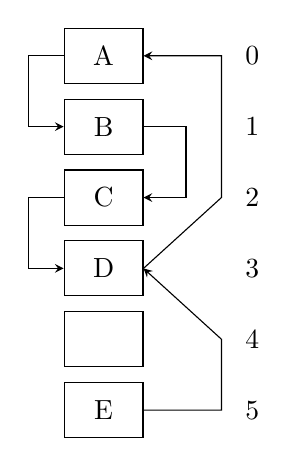
\begin{tikzpicture}[>=stealth,scale=0.9]
  \tikzstyle{slot}=[rectangle,draw,minimum width=1cm,minimum height=0.7cm,inner sep=0pt]

  % Slots (0..5)
  \node[slot] (s0) at (0,0) {A};
  \node[slot] (s1) at (0,-1) {B};
  \node[slot] (s2) at (0,-2) {C};
  \node[slot] (s3) at (0,-3) {D};
  \node[slot] (s4) at (0,-4) {};
  \node[slot] (s5) at (0,-5) {E};

  % Indices
  \node at (2.1,0) {0};
  \node at (2.1,-1) {1};
  \node at (2.1,-2) {2};
  \node at (2.1,-3) {3};
  \node at (2.1,-4) {4};
  \node at (2.1,-5) {5};

  % A: 0 <-> 1
  \draw[->] (s0.west) -- ++(-0.5,0) |- (s1.west);

  % B: 1 <-> 2
  \draw[->] (s1.east) -- ++(0.6,0) |- (s2.east);

  % C: 2 <-> 3
  \draw[->] (s2.west) -- ++(-0.5,0) |- (s3.west);

  % D: 3 <-> 0 (goes upward to avoid colliding with E's arrow)
  \draw[->] (s3.east) -- ++(1.1,1) |- (s0.east);

  % E: 5 <-> 3 (comes from below)
  \draw[->] (s5.east) -- ++(1.1,0) |- ++(0,1) -- (s3.east);
\end{tikzpicture}
\end{center}

We now want to insert a new key \(K\) with possible positions
\begin{align*}
  h_{1}(K) = 5, \qquad h_{2}(K) = 4.
\end{align*}

What is the final state of the hash table after inserting \(K\)?
\oneanswer

\optionsstart
\answer The table ends up as \(\langle A, B, C, D, K, E \rangle\).
\answer The table ends up as \(\langle D, A, B, C, K, E \rangle\). \correct
\answer The table ends up as \(\langle D, A, B, C, E, K \rangle\).
\answer An infinite loop occurs during the insertion, so a rehash will take place.
\optionsend

\explanation{
The insertion proceeds as follows:
\begin{itemize}
  \item \(K\) is inserted at position \(5\),
    so \(E\) is evicted to its alternative position \(3\).
  \item \(E\) is inserted at position \(3\),
    so \(D\) is evicted to its alternative position \(0\).
  \item \(D\) is inserted at position \(0\),
    so \(A\) is evicted to its alternative position \(1\).
  \item \(A\) is inserted at position \(1\),
    so \(B\) is evicted to its alternative position \(2\).
  \item \(B\) is inserted at position \(2\),
    so \(C\) is evicted to its alternative position \(3\).
  \item \(C\) is inserted at position \(3\),
    so \(E\) is evicted to its alternative position \(5\)
  \item \(E\) is inserted at position \(5\),
    so \(K\) is evicted to its alternative position \(4\),
        which is empty.
        Since \(K\) is placed in an empty slot, the insertion stops here.
\end{itemize}
The final table is therefore
\begin{align*}
  \langle D, A, B, C, K, E \rangle.
\end{align*}
}


\question{Functions}
Which of the following functions \(f: \mathbb{R} \to \mathbb{R}\) are bijections?
\multipleanswers

%
\optionsstart
\answer \(x^{2}\)

\answer \(|x|\)

\answer \(x^{3}\) \correct

\answer \(e^{x}\)

\answer \(2x + \sin(x)\) \correct
\optionsend
\explanation{
  \(x^{2}\) is not injective, since \((-1)^2 = 1^2 = 1\).
  \(|x|\) is not injective, since \(|-1|=|1|=1\).
  \(x^{3}\) is both injective and surjective, and hence bijective.
  \(e^{x}\) is not surjective, since there is no \( x \in \mathbb{R}\)
  such that \(e^{x} < 0\).
  \(2x + \sin(x)\) is both injective (since its derivative is \(2 + \cos(x)\geq 1> 0\)) and surjective, and
  hence bijective.
}


\question{Matrix computation}
Let
\begin{align*}
    A =
\begin{bmatrix}
2 & 1\\
0 & 3
\end{bmatrix},\quad
B =
\begin{bmatrix}
1 & 2\\
0 & -1
\end{bmatrix},\quad
C =
\begin{bmatrix}
0 & -2\\
0 & 2
\end{bmatrix}.
\end{align*}
Compute the expression \(A B + A C\).
\oneanswer

\optionsstart
\answer \(\displaystyle
\begin{bmatrix}
2 & 1\\
0 & 3
\end{bmatrix}\) \correct

\answer \(\displaystyle
\begin{bmatrix}
2 & 4\\
0 & -3
\end{bmatrix}\)

\answer \(\displaystyle
\begin{bmatrix}
4 & 2\\
0 & 6
\end{bmatrix}\)

\answer \(\displaystyle
\begin{bmatrix}
1 & 0\\
0 & 1
\end{bmatrix}\)

\optionsend
\explanation{
We can use distributivity:

\begin{align*}
    A B + A C = A(B + C).
\end{align*}

Since \(B + C = I_2\), we get
\begin{align*}
    A(B + C) = A \cdot  I_2 = A.
\end{align*}
Thus

\begin{align*}
A B + A C =
\begin{bmatrix}
2 & 1\\
0 & 3
\end{bmatrix}.
\end{align*}


If we instead compute directly:
\begin{align*}
AB =
\begin{bmatrix}
2 & 1\\
0 & 3
\end{bmatrix}
\begin{bmatrix}
1 & 2\\
0 & -1
\end{bmatrix}
=
\begin{bmatrix}
2 & 3\\
0 & -3
\end{bmatrix},
\quad
AC =
\begin{bmatrix}
2 & 1\\
0 & 3
\end{bmatrix}
\begin{bmatrix}
0 & -2\\
0 & 2
\end{bmatrix}
=
\begin{bmatrix}
0 & -2\\
0 & 6
\end{bmatrix},
\end{align*}

and hence

\begin{align*}
    AB + AC =
\begin{bmatrix}
2 & 3\\
0 & -3
\end{bmatrix}
+
\begin{bmatrix}
0 & -2\\
0 & 6
\end{bmatrix}
=
\begin{bmatrix}
2 & 1\\
0 & 3
\end{bmatrix},
\end{align*}

}


\question{Poker hands}
We play with a standard deck of 52 playing cards (4 suits and 13 ranks).
A hand consists of 5 cards drawn at random without replacement.
How many hands are there of the following type:
\begin{itemize}
\item Three of the cards have the same rank.
\item The remaining two cards have other ranks, but the same suit as each other.
\end{itemize}
\oneanswer

\optionsstart
\answer \(13\cdot \binom{4}{3}\cdot 4\cdot \binom{12}{2}\)\correct
\answer \(13\cdot \binom{4}{3}\cdot 4\cdot 12\cdot 11\) \\
\answer \(13\cdot \binom{4}{3}\cdot \binom{4}{2}\cdot \binom{12}{2}\) \\
\answer \(13\cdot \binom{4}{3}\cdot 4\cdot \binom{13}{2}\)
\optionsend
\explanation{
The three cards of the same rank can be chosen in \(13\cdot \binom{4}{3}\) ways.
The suit of the remaining cards can be chosen in 4 ways, and then we must choose 2 of the 12 remaining ranks.
This gives \(13\cdot \binom{4}{3}\cdot 4\cdot \binom{12}{2}\).
}


\question{Expected Value}
Let \(X_{1}, X_{2}, X_{3}, X_{4}\)
be the outcomes of four independent rolls of a standard six-sided die.
What is the expected value of \((X_{1} + X_{2})\cdot (X_{3}+X_{4})\)?
\oneanswer

\optionsstart
\answer 24
\answer 28
\answer 36
\answer 49 \correct
\answer 64
\optionsend
\explanation{Since \(X_{1} + X_{2}\) and \(X_{3} + X_{4}\) depend on
  different die rolls, they are independent, so the expected value is the product of their expected values:
  \begin{align*}
    \mathbb{E}[(X_{1} + X_{2}) \cdot ( X_{3} + X_{4})] =
    \mathbb{E}[X_{1} + X_{2}] \cdot \mathbb{E}[ X_{3} + X_{4}] =
    (\mathbb{E}[X_{1}] + \mathbb{E}[X_{2}]) \cdot (\mathbb{E}[ X_{3}] + \mathbb{E}[X_{4}])
  \end{align*}
  Since the expected value of a single roll of a six-sided die is
  \begin{align*}
      \mathbb{E}[X_{i}] &=
      \frac{1+2+3+4+5+6}{6} = 3.5
  \end{align*}
  we get the result
  \begin{align*}
    \left( 3.5 + 3.5\right)^{2} = 7^{2} = 49.
  \end{align*}
}



\question{Dijkstra's algorithm}
Consider the following weighted, directed graph:

\begin{center}
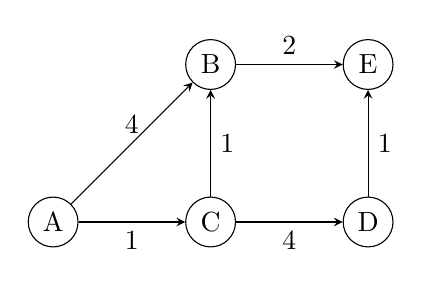
\begin{tikzpicture}[>=stealth, node distance=2.4cm]
  \tikzstyle{vertex}=[circle,draw,minimum size=18pt,inner sep=0pt]

  \node[vertex] (A) at (0,-2) {A};
  \node[vertex] (B) at (2,0) {B};
  \node[vertex] (C) at (2,-2) {C};
  \node[vertex] (D) at (4,-2) {D};
  \node[vertex] (E) at (4,0) {E};

  \draw[->] (A) -- node[above] {4} (B);
  \draw[->] (A) -- node[below] {1} (C);
  \draw[->] (C) -- node[right] {1} (B);
  \draw[->] (C) -- node[below] {4} (D);
  \draw[->] (B) -- node[above] {2} (E);
  \draw[->] (D) -- node[right] {1} (E);
\end{tikzpicture}
\end{center}

Suppose Dijkstra's algorithm is used to find the shortest distances from vertex \(A\)
to all vertices in the graph. State the order in which the vertices are extracted from
the priority queue in Dijkstra's algorithm.
\oneanswer

\optionsstart
\answer \(A C B E D\) \correct
\answer \(A B C E D\)
\answer \(A C B D E\)
\answer \(A C D B E\)
\optionsend
\explanation{
  \begin{itemize}
      \item Start: \(d(A)=0\), all others \(\infty\).
      \item From \(A\): \(d(B)=4\), \(d(C)=1\). The next vertex is \(C\) (smallest distance).
\item From \(C\): \(d(B)\) is improved to \(1+1=2\), \(d(D)=1+4=5\).
\item The next vertex is \(B\) (distance \(2\)), which gives \(d(E)=1+1+2=4\).
\item The next vertex is \(E\) (distance \(4\)).
\item The last vertex is \(D\) (distance \(5\)).
\end{itemize}
The order is therefore \(A,C,B,E,D\).
}


\question{Recurrence}
Consider the following recurrence:
\begin{align*}
    T(0) & = 1 \\
    T(n) & = 2T(n-1) + 1 \quad \text{for } n \geq 1.
\end{align*}
Which of the following functions solves the recurrence?
\oneanswer

\optionsstart
\answer \(2^{n+1}-1\) \correct
\answer \(2n +1\)
\answer \(3 \cdot 2^{n}-1\)
\answer \(2^{n}+n\)
\optionsend
\explanation{
We have \(2^{0+1}-1 = 1\), so \(2^{n+1}-1\) satisfies the initial condition.
Furthermore, we see that
\begin{align*}
    2^{n+1}-1 = 2 \cdot 2^{n} - 1 = 2 \cdot \left( 2^{n} - 1\right) + 1,
\end{align*}
which shows that the function satisfies the recurrence.
}




\multiplechoiceend

\label{page:last}
